\documentclass[conference,10pt]{IEEEtran}

\usepackage[utf8]{inputenc}
\usepackage[T1]{fontenc}
\usepackage[spanish,es-nodecimaldot,es-noshorthands,es-tabla]{babel}
\usepackage{amsmath,amssymb}
\usepackage{graphicx}
\usepackage{booktabs}
\usepackage{multirow}
\usepackage{cite}
\usepackage{url}
\usepackage{algorithm}
\usepackage{algpseudocode}
\usepackage{microtype}
\usepackage{balance}

\renewcommand{\IEEEkeywordsname}{Palabras clave}
\floatname{algorithm}{Algoritmo}
\algrenewcommand\algorithmicwhile{\textbf{mientras}}
\algrenewcommand\algorithmicdo{\textbf{hacer}}
\algrenewcommand\algorithmicfor{\textbf{para}}
\algrenewcommand\algorithmicif{\textbf{si}}
\algrenewcommand\algorithmicthen{\textbf{entonces}}
\algrenewcommand\algorithmicend{\textbf{fin}}
\algrenewcommand\algorithmicreturn{\textbf{devolver}}
\newcommand{\x}{$\times$}

\begin{document}

\title{Búsqueda en GPU sobre los grafos de ParlayANN:\\
aceleración con resultados idénticos a la CPU}

\author{
\IEEEauthorblockN{Samuel Iman Quispe, Juan Victor Tejeda y Jean Marc Nadeau Huamani}
\IEEEauthorblockA{Escuela Profesional de Ciencia de la Computación\\
Universidad Católica San Pablo (UCSP), Arequipa, Perú\\
Curso de Computación Paralela}
}

\maketitle

\begin{abstract}
ParlayANN implementa versiones paralelas y deterministas de cuatro algoritmos de
búsqueda aproximada de vecinos más cercanos basados en grafos (DiskANN, HCNNG,
PyNNDescent y HNSW), pero solo para CPU multinúcleo. En este trabajo implementamos en
CUDA la búsqueda de los cuatro algoritmos sobre \emph{los mismos grafos} que construye
ParlayANN, reproduciendo paso a paso su lógica, de modo que la GPU devuelve los mismos
vecinos que la CPU. Esto permite medir el beneficio de la GPU sin mezclarlo con cambios
de algoritmo. Sobre MSSPACEV-1M (un millón de vectores) y en dos laptops de distinta
generación, la GPU reproduce el recall de la CPU en las 72 configuraciones evaluadas,
devuelve los mismos 10 vecinos en el 100\,\% de las consultas de DiskANN, HCNNG y
PyNNDescent (en HNSW, las mismas distancias), y es determinista. Con recall@10 $\geq$
0,95, la búsqueda en GPU es entre 3,7\x{} y 7,2\x{} más rápida que la CPU en una laptop
con i5-12450HX y RTX~3050, y entre 6,6\x{} y 10,7\x{} en otra con i7-13700HX y RTX~5050.
Mostramos que el kernel está limitado por el acceso aleatorio a memoria y que, entre
generaciones, la GPU mejoró bastante más que la CPU.
\end{abstract}

\begin{IEEEkeywords}
búsqueda de vecinos más cercanos, grafos de proximidad, GPU, CUDA, ParlayANN,
reproducibilidad
\end{IEEEkeywords}

% ============================================================================
\section{Introducción}

La búsqueda aproximada de vecinos más cercanos (ANNS) es una pieza central de los
sistemas de recomendación, la recuperación de información y las bases de datos
vectoriales. Entre los métodos existentes, los basados en grafos de proximidad obtienen
la mejor relación entre recall y consultas por segundo (QPS)~\cite{wang2021graphsurvey,aumuller2020annbenchmarks}.
ParlayANN~\cite{manohar2024parlayann} reúne implementaciones paralelas, sin bloqueos y
deterministas de DiskANN~\cite{subramanya2019diskann}, HCNNG~\cite{munoz2019hcnng},
PyNNDescent~\cite{mcinnes2020pynndescent} y HNSW~\cite{malkov2020hnsw}, pero solo para
CPU multinúcleo.

Los trabajos de ANNS en GPU~\cite{zhao2020song,groh2023ggnn,yu2022ganns,ootomo2024cagra,karthik2024bang}
persiguen el mejor compromiso recall--QPS en ese hardware y, para lograrlo, cambian la
búsqueda, el grafo o la representación de los vectores. Por eso, al compararlos con una
CPU es difícil separar cuánto aporta el hardware y cuánto el algoritmo distinto.

Nuestro objetivo es otro: tomar los grafos que construye ParlayANN y ejecutar \emph{la
misma búsqueda} en una GPU. Las contribuciones son:
\begin{itemize}
\item Un kernel CUDA de búsqueda para los cuatro algoritmos de ParlayANN que reproduce su
lógica exacta, incluidas sus particularidades (filtro de visitados con pérdidas, aristas
repetidas, candidatos de HNSW ordenados solo por distancia).
\item Una validación vecino por vecino contra la CPU en 72 configuraciones y una
verificación de determinismo.
\item Una evaluación en dos laptops de distinta generación que muestra cuánto acelera la
GPU, qué la limita y cómo cambia la ventaja con el hardware.
\end{itemize}

% ============================================================================
\section{Antecedentes y trabajo relacionado}

\subsection{Búsqueda en grafos y ParlayANN}

Un índice basado en grafos conecta cada punto con algunos vecinos cercanos y responde una
consulta con una \emph{beam search} (Algoritmo~\ref{alg:beam}): se mantiene una frontera
con los $L_s$ mejores candidatos, se expande el más cercano aún no visitado, se calculan
las distancias de sus vecinos y se mezclan con la frontera, hasta que todos los puntos de
la frontera fueron visitados. El parámetro $L_s$ controla el compromiso entre recall y
velocidad. DiskANN construye el grafo Vamana con inserciones y poda $\alpha$; HCNNG une
árboles de expansión mínima de muchos agrupamientos jerárquicos; PyNNDescent refina un
grafo inicial con vecinos de vecinos~\cite{dong2011nndescent}, y HNSW organiza grafos en
varios niveles y desciende por ellos antes de buscar en el nivel 0.

ParlayANN~\cite{manohar2024parlayann} paraleliza la \emph{construcción} de estos grafos
con inserción por lotes con \emph{prefix doubling} y ordenamientos en lugar de bloqueos,
usando ParlayLib~\cite{blelloch2020parlaylib}, y lo hace de forma determinista. En la
búsqueda, cada hilo resuelve consultas distintas.

\begin{algorithm}[t]
\caption{Beam search de ParlayANN (simplificada)}
\label{alg:beam}
\begin{algorithmic}[1]
\State $F \gets \{(0, d(q,p_0))\}$; $V \gets \emptyset$ \Comment{frontera y visitados}
\While{existe $u \in F \setminus V$}
  \State $u \gets$ el más cercano de $F \setminus V$; $V \gets V \cup \{u\}$
  \State $C \gets$ vecinos de $u$ que no pasaron por el filtro hash
  \State calcular $d(q,c)$ para cada $c \in C$
  \State $F \gets$ los $L_s$ mejores de $F \cup C$ \Comment{orden (distancia, id)}
  \State recortar $F$ a distancias $\leq 1{,}35 \cdot d_k$
\EndWhile
\State \Return los $k$ primeros de $F$
\end{algorithmic}
\end{algorithm}

\subsection{ANNS en GPU}

FAISS~\cite{johnson2021faiss} acelera en GPU la búsqueda por cuantización e índices
invertidos. SONG~\cite{zhao2020song} fue de los primeros en llevar la búsqueda en grafos
a la GPU; GGNN~\cite{groh2023ggnn} y GANNS~\cite{yu2022ganns} diseñan grafos y búsquedas
adaptadas a ella, y CAGRA~\cite{ootomo2024cagra} reporta entre 33\x{} y 77\x{} más QPS
que HNSW en lotes grandes. BANG~\cite{karthik2024bang} busca sobre el grafo de DiskANN
con vectores comprimidos para escalar a miles de millones de puntos. En CPU,
iQAN~\cite{peng2023iqan} explora el paralelismo dentro de una misma consulta. A
diferencia de estos trabajos, no proponemos un algoritmo nuevo: reproducimos el de
ParlayANN para aislar el efecto del hardware.

% ============================================================================
\section{Diseño de la búsqueda en GPU}

\subsection{Organización del trabajo}

Cada consulta la resuelve un \emph{warp} de 32 hilos. Se lanzan solo los warps que caben
a la vez en la GPU, y cada uno toma consultas de forma estática ($q$, $q+W$, \dots), lo que
evita atómicos y hace el resultado independiente del planificador. La frontera, los
candidatos y la consulta viven en memoria compartida; el filtro de visitados y la tabla
de visitados, en memoria global, una región por warp. Los vectores int8 de 100
dimensiones se rellenan a 128 bytes y el grafo se guarda como una matriz
$n \times \text{grado}_{\max}$, de modo que la fila de un nodo se lee sin indirecciones.

La distancia euclidiana al cuadrado se calcula como
$\lVert q-p\rVert^2 = \lVert q\rVert^2 + \lVert p\rVert^2 - 2\,q\cdot p$, con las normas
precalculadas y el producto punto con la instrucción \texttt{\_\_dp4a}, que multiplica y
suma cuatro pares de bytes. Toda la aritmética es entera, así que el resultado es el
mismo número que calcula ParlayANN.

\subsection{Reproducir exactamente la CPU}

Para devolver los mismos vecinos hay que copiar también los detalles del código original:
\begin{itemize}
\item La búsqueda empieza en el punto 0, con $k=10$ y corte $1{,}35\,d_k$; el umbral se
calcula en doble precisión y se compara en simple, como en C++.
\item El filtro de ``ya visto'' es una tabla hash con pérdidas
(\texttt{hash64\_2} de ParlayLib) en la que cada vecino puede pisar la casilla de otro.
En la CPU se revisan en orden; en la GPU, los 32 hilos leen todas las casillas de una vez
y, con \texttt{\_\_match\_any\_sync} y una búsqueda hacia atrás en memoria compartida,
cada hilo determina qué había en su casilla justo antes de él. Así el resultado es el
mismo que el secuencial.
\item El grafo de HCNNG tiene 26,9 millones de aristas repetidas (27\,\%) y el de
PyNNDescent 5\,637. La unión de la frontera con los candidatos se trata como un
multiconjunto, igual que \texttt{std::set\_union}.
\item En HNSW, los candidatos se guardan en un \texttt{std::set} ordenado solo por
distancia (si ya hay uno con la misma distancia, el nuevo no entra) y aceptar un vecino
cambia el umbral del siguiente. Esa decisión se toma en orden, mientras que leer la fila,
filtrar, calcular distancias y desplazar los arreglos ordenados se hace con los 32 hilos.
\end{itemize}

\subsection{Optimizaciones}

La primera versión asignaba una distancia a cada hilo, que leía su propio vector de 128
bytes. Un microbenchmark (Tabla~\ref{tab:micro}) mostró que leer cada vector con 8 hilos
a la vez es 3,75\x{} más rápido en la RTX~3050. La versión final:
(i)~calcula cada distancia con un grupo de 8 hilos y cada hilo lleva 4 distancias, de modo
que un warp tiene 16 vectores pedidos a memoria al mismo tiempo; (ii)~lee la fila de
vecinos completa y todas las casillas del filtro en un solo viaje a memoria, en lugar de
uno por cada 32 vecinos, y (iii)~reutiliza arreglos de memoria compartida para que entren
más warps por SM. La Tabla~\ref{tab:opt} resume el efecto.

También probamos guardar una \emph{época} en cada casilla del filtro para no limpiarlo en
cada consulta. Daba el mismo resultado, pero fue 30\,\% más lento: limpiar escribe líneas
completas que quedan en la caché L2, mientras que con épocas las lecturas iban a memoria
principal y las casillas pasaban de 4 a 8 bytes. La descartamos en DiskANN, HCNNG y
PyNNDescent; en HNSW la mantenemos porque hay una tabla por nivel.

\begin{table}[t]
\centering
\caption{Efecto de las optimizaciones (RTX~3050, DiskANN, $L_s=75$, recall 0,955;
QPS solo del kernel)}
\label{tab:opt}
\begin{tabular}{lrr}
\toprule
Versión & QPS & vs.\ CPU \\
\midrule
CPU, 12 hilos (ParlayANN) & 32\,079 & 1,00\x \\
1 hilo por distancia & 42\,856 & 1,34\x \\
+ 8 hilos por vector & 56\,781 & 1,77\x \\
+ lecturas agrupadas y más warps (final) & 141\,071 & 4,40\x \\
\midrule
Final con épocas (descartada) & 98\,320 & 3,06\x \\
\bottomrule
\end{tabular}
\end{table}

% ============================================================================
\section{Metodología experimental}

\textbf{Datos y configuraciones.} Usamos MSSPACEV-1M~\cite{spacev1b,simhadri2022bigann}:
un millón de vectores int8 de 100 dimensiones, 29\,316 consultas y $k=10$. Los cuatro
grafos los construye ParlayANN (commit \texttt{45587ba}) con los parámetros de su
artefacto: DiskANN con $R=64$, $L=128$, $\alpha=1{,}2$; HCNNG con 50 árboles y hojas de
1000 puntos; PyNNDescent con grado 60, y HNSW con $m=32$, $ef_c=128$. Cada algoritmo se
evalúa en las mismas 18 configuraciones de búsqueda: $L_s=10$ con un límite de 3, 5, 8, 12
o 15 nodos visitados, y $L_s \in \{15, 20, 30, 40, 50, 60, 75, 100, 150, 200, 400, 500,
1000\}$.

\textbf{Plataformas.} La Tabla~\ref{tab:plataformas} resume las dos laptops. La CPU usa
todos sus hilos y corre en WSL2 con big-ann-benchmarks~\cite{simhadri2022bigann}; la GPU,
en Windows con CUDA. Ambas estaban conectadas a la corriente y en el modo de energía de
máximo rendimiento.

\begin{table}[t]
\centering
\caption{Plataformas}
\label{tab:plataformas}
\begin{tabular}{lll}
\toprule
 & Máquina A & Máquina B \\
\midrule
CPU & i5-12450HX & i7-13700HX \\
Núcleos / hilos & 8 (4P+4E) / 12 & 16 (8P+8E) / 24 \\
RAM & 24 GB DDR5-4800 & 16 GB DDR5-4800 \\
GPU & RTX 3050 Laptop & RTX 5050 Laptop \\
Arquitectura & Ampere (\texttt{sm\_86}) & Blackwell (\texttt{sm\_120}) \\
SM / VRAM & 20 / 6 GB & 20 / 8 GB \\
CUDA & 12.9 & 12.8 \\
\bottomrule
\end{tabular}
\end{table}

\textbf{Protocolo.} En los dos lados se hace una corrida de calentamiento y se toma la
mejor de cinco, como en big-ann-benchmarks. En la CPU se mide la llamada de búsqueda del
benchmark; en la GPU, \emph{de punta a punta}: copiar las consultas, calcular sus normas,
ejecutar el kernel y traer ids y distancias. También reportamos el tiempo solo del kernel.
La carga del índice no se cuenta en ningún lado. El recall@10 se calcula como en
big-ann-benchmarks, contando los empates de distancia del vecino $k$-ésimo.

\textbf{Validación.} Para cada configuración comparamos, consulta por consulta, los
vecinos de la GPU con los que guardó la CPU, y las distancias cuando los ids difieren.
Además, comprobamos que la corrida de calentamiento y la última devuelvan exactamente lo
mismo (determinismo). Las consultas en las que la frontera termina con menos de 10
elementos se excluyen de la comparación vecino por vecino, porque ahí la CPU devuelve
memoria sin inicializar (entre 0 y 163 de 527\,688 por algoritmo).

% ============================================================================
\section{Resultados}

\subsection{Exactitud}

En las dos máquinas, las 72 configuraciones dan el mismo recall que la CPU y son
deterministas (Tabla~\ref{tab:exactitud}). En DiskANN, HCNNG y PyNNDescent la GPU
devuelve exactamente los mismos 10 vecinos en todas las consultas. En HNSW coinciden en
el 99,4\,\% de las consultas; en el resto, los vecinos distintos están \emph{a la misma
distancia} que los de la CPU. Son empates que el heap de la CPU resuelve de otra forma, y
no cambian el recall.

\begin{table}[t]
\centering
\caption{Exactitud de la GPU frente a la CPU (18 configuraciones por algoritmo)}
\label{tab:exactitud}
\begin{tabular}{lcccc}
\toprule
 & Recall & \multicolumn{2}{c}{Mismos 10 vecinos} & Mismas \\
Algoritmo & idéntico & A & B & distancias \\
\midrule
DiskANN & 18/18 & 100\,\% & 100\,\% & 100\,\% \\
HCNNG & 18/18 & 100\,\% & 100\,\% & 100\,\% \\
PyNNDescent & 18/18 & 100\,\% & 100\,\% & 100\,\% \\
HNSW & 18/18 & 99,42\,\% & 99,44\,\% & 100\,\% \\
\bottomrule
\end{tabular}
\end{table}

\subsection{Rendimiento}

La Tabla~\ref{tab:qps} compara el mejor QPS que alcanza cada lado con un recall mínimo, y
la Fig.~\ref{fig:speedup} resume el caso de recall $\geq 0{,}95$. La GPU es más rápida en
todas las configuraciones: entre 2,5\x{} y 14,5\x{} en la máquina A y entre 3,0\x{} y
12,2\x{} en la B. La Fig.~\ref{fig:curvas} muestra las curvas recall--QPS completas de
DiskANN y HNSW.

\begin{table*}[t]
\centering
\caption{Mejor QPS que cumple cada recall@10 mínimo (GPU de punta a punta) y speedup GPU/CPU}
\label{tab:qps}
\begin{tabular}{llrrrrrrrr}
\toprule
 & & \multicolumn{3}{c}{Máquina A (i5 + RTX 3050)} & \multicolumn{3}{c}{Máquina B (i7 + RTX 5050)}
 & \multicolumn{2}{c}{Mejora B/A} \\
\cmidrule(lr){3-5}\cmidrule(lr){6-8}\cmidrule(lr){9-10}
Recall & Algoritmo & CPU & GPU & Speedup & CPU & GPU & Speedup & CPU & GPU \\
\midrule
\multirow{4}{*}{$\geq 0{,}90$}
 & DiskANN     & 74\,473 & 344\,395 & 4,6\x  & 107\,770 & 1\,261\,511 & 11,7\x & 1,45\x & 3,66\x \\
 & HCNNG       & 35\,552 & 167\,164 & 4,7\x  & 50\,912  & 517\,290    & 10,2\x & 1,43\x & 3,09\x \\
 & PyNNDescent & 72\,518 & 330\,460 & 4,6\x  & 100\,805 & 1\,058\,687 & 10,5\x & 1,39\x & 3,20\x \\
 & HNSW        & 17\,853 & 192\,328 & 10,8\x & 41\,249  & 385\,865    & 9,4\x  & 2,31\x & 2,01\x \\
\midrule
\multirow{4}{*}{$\geq 0{,}95$}
 & DiskANN     & 32\,079 & 140\,531 & 4,4\x  & 52\,325  & 561\,297    & 10,7\x & 1,63\x & 3,99\x \\
 & HCNNG       & 19\,936 & 74\,808  & 3,8\x  & 28\,150  & 251\,385    & 8,9\x  & 1,41\x & 3,36\x \\
 & PyNNDescent & 44\,258 & 163\,524 & 3,7\x  & 62\,352  & 605\,957    & 9,7\x  & 1,41\x & 3,71\x \\
 & HNSW        & 7\,350  & 52\,635  & 7,2\x  & 16\,530  & 108\,921    & 6,6\x  & 2,25\x & 2,07\x \\
\midrule
\multirow{4}{*}{$\geq 0{,}98$}
 & DiskANN     & 7\,920  & 23\,350  & 2,9\x  & 12\,482  & 62\,493     & 5,0\x  & 1,58\x & 2,68\x \\
 & HCNNG       & 10\,509 & 27\,754  & 2,6\x  & 16\,226  & 108\,498    & 6,7\x  & 1,54\x & 3,91\x \\
 & PyNNDescent & 18\,253 & 48\,795  & 2,7\x  & 27\,658  & 196\,575    & 7,1\x  & 1,52\x & 4,03\x \\
 & HNSW        & 1\,348  & 6\,149   & 4,6\x  & 5\,291   & 31\,841     & 6,0\x  & 3,93\x & 5,18\x \\
\bottomrule
\end{tabular}
\end{table*}

\begin{figure}[t]
\centering
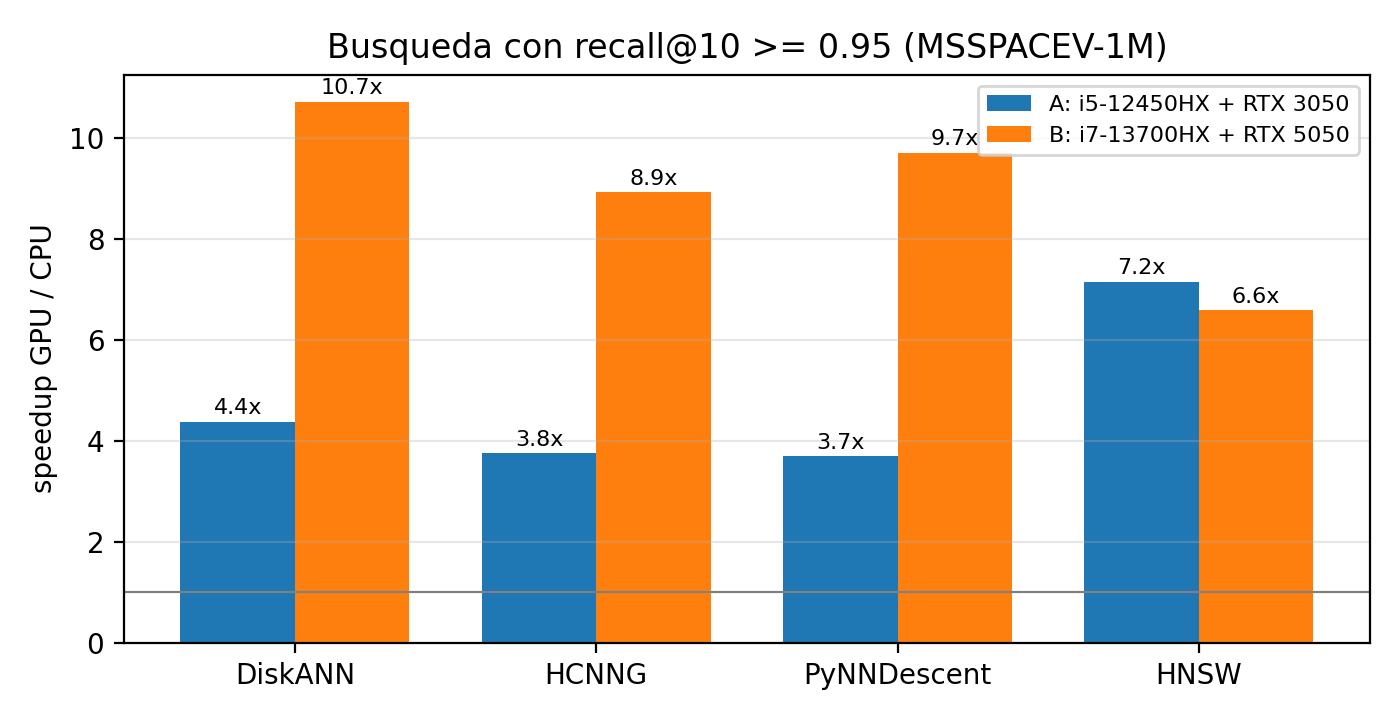
\includegraphics[width=\columnwidth]{figuras/speedup_maquinas.png}
\caption{Speedup de la búsqueda en GPU con recall@10 $\geq 0{,}95$ (de punta a punta).}
\label{fig:speedup}
\end{figure}

\begin{figure*}[t]
\centering
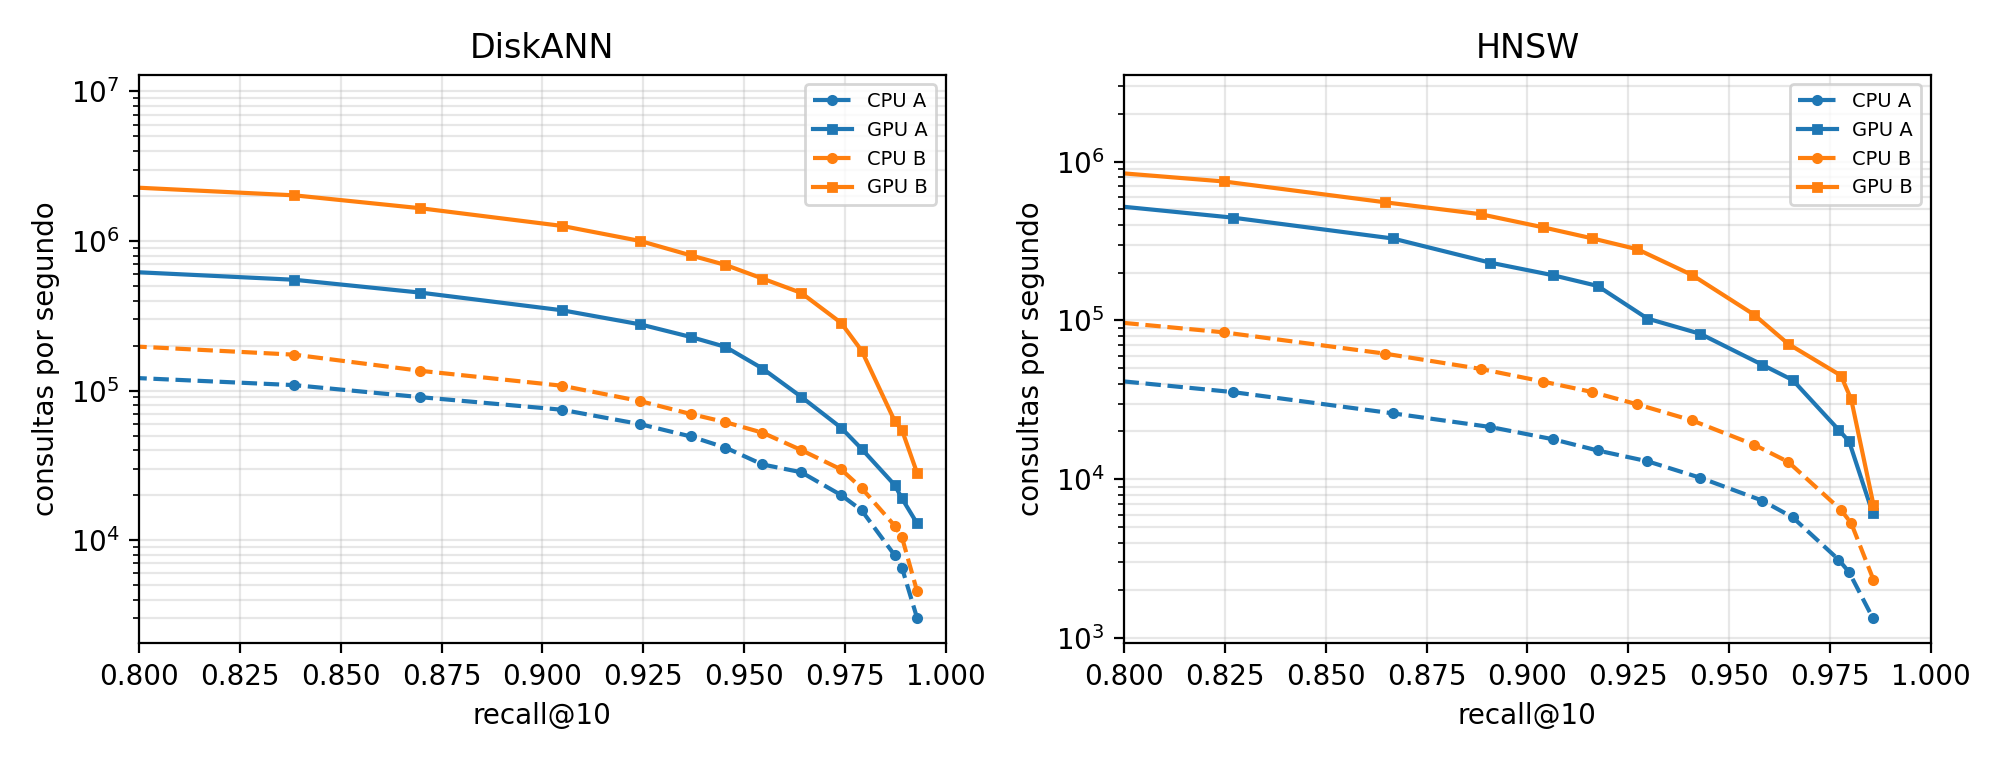
\includegraphics[width=0.85\textwidth]{figuras/recall_qps_maquinas.png}
\caption{Recall@10 frente a QPS (escala logarítmica) de DiskANN y HNSW en las dos
máquinas. Líneas punteadas: CPU; continuas: GPU de punta a punta.}
\label{fig:curvas}
\end{figure*}

El costo de mover datos entre la CPU y la GPU es pequeño: con recall $\geq 0{,}95$, el QPS
de punta a punta está a menos del 2\,\% del QPS del kernel. Solo en las configuraciones
más rápidas (más de un millón de consultas por segundo), la copia llega a pesar entre 10 y
15\,\%.

\subsection{Qué limita al kernel}

La Tabla~\ref{tab:micro} muestra el microbenchmark de distancias a puntos aleatorios y el
reparto del tiempo del kernel, medido con \texttt{clock64()} dentro de cada sección. En la
RTX~3050, DiskANN con $L_s=75$ calcula 499 millones de distancias por segundo, el 90\,\%
del máximo que alcanza el microbenchmark (555 millones): el kernel está limitado por el
acceso aleatorio a memoria, y las distancias son casi la mitad de su tiempo. En la
RTX~5050 calcula 2\,026 millones por segundo (78\,\% del máximo) y las distancias bajan al
28\,\%: con más ancho de banda, empiezan a pesar las partes con menos paralelismo
(ordenar candidatos, la unión con la frontera y el corte).

\begin{table}[t]
\centering
\caption{Microbenchmark de distancias (millones por segundo) y reparto del tiempo del
kernel (DiskANN, $L_s=75$)}
\label{tab:micro}
\begin{tabular}{lrr}
\toprule
 & RTX 3050 & RTX 5050 \\
\midrule
1 hilo por distancia & 148 & 568 \\
1 warp por distancia & 527 & 996 \\
8 hilos por distancia (usada) & 555 & 2\,590 \\
\midrule
Distancias en el kernel & 48,0\,\% & 28,1\,\% \\
Leer vecinos y filtro & 24,2\,\% & 21,0\,\% \\
Unión con la frontera & 10,2\,\% & 13,7\,\% \\
Ordenar candidatos & 3,0\,\% & 13,1\,\% \\
Corte y siguiente nodo & 4,3\,\% & 11,0\,\% \\
Otros & 10,3\,\% & 13,1\,\% \\
\bottomrule
\end{tabular}
\end{table}

% ============================================================================
\section{Discusión}

\textbf{La GPU mejoró más que la CPU entre generaciones.} Con recall $\geq 0{,}95$, la CPU
de la máquina B es entre 1,4\x{} y 1,6\x{} más rápida que la de A, aunque tiene el doble
de hilos, mientras que la GPU es entre 3,4\x{} y 4,0\x{} más rápida en DiskANN, HCNNG y
PyNNDescent. Coincide con el microbenchmark: la RTX~5050 calcula 4,7\x{} más distancias
por segundo. Por eso el speedup pasa de unas 4\x{} a unas 10\x. La búsqueda en grafos está
dominada por accesos aleatorios a memoria, y ahí las GPU de laptop crecieron más rápido.

\textbf{HNSW escala distinto.} Su GPU mejoró solo 2\x{} entre máquinas y, con $L_s=1000$,
el speedup baja a 4,6\x{} en A y 3,0\x{} en B. En HNSW, aceptar un vecino cambia el umbral
del siguiente, así que esa decisión es secuencial, y desplazar los arreglos ordenados
crece con el tamaño del \emph{workset}; esas partes no aprovechan el mayor ancho de banda.
En la máquina A, HNSW muestra el mayor speedup porque su versión de CPU es la más lenta.

\textbf{Comparación entre máquinas.} Los grafos de DiskANN construidos en las dos
máquinas son iguales (el recall de la CPU coincide en las 18 configuraciones), pero los de
HCNNG, PyNNDescent y HNSW no (el recall difiere hasta en 0,015). Cada máquina los
construyó con su número de hilos (12 y 24), así que no podemos atribuir la diferencia a
una causa. El speedup dentro de cada máquina es exacto, porque CPU y GPU usan el mismo
grafo; para comparar generaciones, DiskANN es el caso más limpio.

\textbf{Limitaciones.} Evaluamos un solo conjunto de datos de un millón de puntos, en
laptops, donde la temperatura y el modo de energía influyen. La CPU corre en WSL2 y la GPU
en Windows nativo. La construcción de los grafos sigue en la CPU.

% ============================================================================
\section{Conclusiones y trabajo futuro}

Implementamos en CUDA la búsqueda de los cuatro algoritmos de ParlayANN sobre sus propios
grafos, con resultados idénticos a los de la CPU y deterministas en las 72 configuraciones
evaluadas. Esta equivalencia permite atribuir la diferencia de rendimiento solo al
hardware: con recall $\geq 0{,}95$ la GPU es entre 3,7\x{} y 7,2\x{} más rápida en una
laptop con RTX~3050 y entre 6,6\x{} y 10,7\x{} con una RTX~5050. El kernel está limitado
por el acceso aleatorio a memoria; leer cada vector con 8 hilos fue la optimización
decisiva, y guardar épocas en el filtro, aunque parecía útil, resultó más lento. Como
trabajo futuro, queda llevar a la GPU la construcción de los grafos (empezando por la
inserción por lotes de DiskANN y HNSW), evaluar conjuntos de datos más grandes y reducir
la parte secuencial de HNSW.

\balance
\bibliographystyle{IEEEtran}
\bibliography{referencias}

\end{document}
